\chapter{The Assignment Operator and Defining Functions}
\label{chp:assignment_operator}

\section{Assigning Expressions}
\label{sec:assigning_expressions}

Having to retype the same expression multiple times is tedious, but using copy and paste in Maple can sometimes produce unwanted effects. A better way to reuse an expression multiple times is to assign a name to it. You can assign any expression to a name of your choice (with some exceptions that Maple has protected) by using the \text{:=} operator.
\index{assignment operator}
\index{mathematical functions!exponential}
\index{mathematical functions!square root}
\marginnote{Protected names include common functions such as \texttt{exp}. For example, \begin{center}\texttt{> exp := 2*x;}\end{center} would cause an error.}

\begin{maplegroup}
\begin{mapleinput}
\mapleinline{active}{1d}{poly := 3*x\symbol{94}4 - 2*x + 1;
}{}
\end{mapleinput}
\mapleresult
\begin{maplelatex}
\mapleinline{inert}{2d}{poly := 3*x^4-2*x+1}{\[\displaystyle {\it poly}\, := \,3\,{x}^{4}-2\,x+1\]}
\end{maplelatex}
\end{maplegroup}

\begin{maplegroup}
\begin{mapleinput}
\mapleinline{active}{1d}{poly;
}{}
\end{mapleinput}
\mapleresult
\begin{maplelatex}
\mapleinline{inert}{2d}{3*x^4-2*x+1}{\[\displaystyle 3\,{x}^{4}-2\,x+1\]}
\end{maplelatex}
\end{maplegroup}

\marginnote[0.5cm]{Never assign anything to single-letter names such as $x$ or $y$. It is best to keep single letters as arbitrary variables.}
\begin{maplegroup}
\begin{mapleinput}
\mapleinline{active}{1d}{poly\symbol{94}2;
}{}
\end{mapleinput}
\mapleresult
\begin{maplelatex}
\mapleinline{inert}{2d}{(3*x^4-2*x+1)^2}{\[\displaystyle  \left( 3\,{x}^{4}-2\,x+1 \right) ^{2}\]}
\end{maplelatex}
\end{maplegroup}

\begin{maplegroup}
\begin{mapleinput}
\mapleinline{active}{1d}{expr := (4\symbol{94}x - x\symbol{94}4) / exp(x + 1);
}{}
\end{mapleinput}
\mapleresult
\begin{maplelatex}
\mapleinline{inert}{2d}{expr:=(4^x-x^4)/exp(x+1)}{\[\displaystyle {\it expr}\, := \,{\frac {{4}^{x}-{x}^{4}}{{{\rm e}^{x+1}}}}\]}
\end{maplelatex}
\end{maplegroup}

\marginnote{It is important to assign expressions to names that make sense to you and are easy to remember. It is also recommended not to reuse a name in the same document. If you assign a new expression to an old name, the new expression will overwrite what was previously assigned.}
\begin{maplegroup}
\begin{mapleinput}
\mapleinline{active}{1d}{expr;
}{}
\end{mapleinput}
\mapleresult
\begin{maplelatex}
\mapleinline{inert}{2d}{(4^x-x^4)/exp(x+1)}{\[\displaystyle {\frac {{4}^{x}-{x}^{4}}{{{\rm e}^{x+1}}}}\]}
\end{maplelatex}
\end{maplegroup}

\begin{maplegroup}
\begin{mapleinput}
\mapleinline{active}{1d}{sqrt(expr);
}{}
\end{mapleinput}
\mapleresult
\begin{maplelatex}
\mapleinline{inert}{2d}{sqrt((4^x-x^4)/exp(x+1))}{\[\displaystyle  \sqrt{{\frac {{4}^{x}-{x}^{4}}{{{\rm e}^{x+1}}}}}\]}
\end{maplelatex}
\end{maplegroup}

\section{Making a Substitution into an Expression}
\label{sec:making_substitutions}

Let's suppose you have assigned an expression a name, and wish to replace one of its variables with a value or expression. As an example, we will assign an expression a name of \texttt{expr} and then substitute the numerical value for $\pi$, which is denoted as \texttt{Pi} in Maple, into \texttt{expr}. The command used to substitute a value into an expression is \texttt{subs()}.

\begin{maplegroup}
\begin{mapleinput}
\mapleinline{active}{1d}{expr := sin(x) - 1;
}{}
\end{mapleinput}
\mapleresult
\begin{maplelatex}
\mapleinline{inert}{2d}{expr := sin(x)-1}{\[\displaystyle {\it expr}\, := \,\sin \left( x \right) -1\]}
\end{maplelatex}
\end{maplegroup}
\marginnote[-.2cm]{Always be sure to use a capital P in \texttt{Pi} for the mathematical constant. You can also find $\pi$ in the palettes toolbar.}
\index{Pi}
\index{mathematical functions!sine}
\index{mathematical functions!exponential}
\index{ditto operator}
\index{mathematical functions!tangent}


\begin{maplegroup}
\begin{mapleinput}
\mapleinline{active}{1d}{subs(x = Pi, expr);
}{}
\end{mapleinput}
\mapleresult
\begin{maplelatex}
\mapleinline{inert}{2d}{sin(Pi)-1}{\[\displaystyle \sin \left( \pi  \right) -1\]}
\end{maplelatex}
\end{maplegroup}
\marginnote[0.1cm]{The order of the parameters in the \texttt{subs()} command is important. For example, \begin{center}\texttt{> subs(expr,x = Pi);}\end{center} would cause an error.}
You can make use of the \% shortcut if you wish, but recall that it is best used on the same Maple input:

\begin{maplegroup}
\begin{mapleinput}
\mapleinline{active}{1d}{x\symbol{94}2 + 3*x - 4; subs(x = 2, %);
}{}
\end{mapleinput}
\mapleresult\begin{maplelatex}
\mapleinline{inert}{2d}{x^2+3*x-4}{\[\displaystyle {x}^{2}+3\,x-4\]}
\end{maplelatex}
\begin{maplelatex}
\mapleinline{inert}{2d}{6}{\[\displaystyle 6\]}
\end{maplelatex}
\end{maplegroup}



You can also substitute one expression into another:
\marginnote{Note that using the \texttt{subs()} command does not permanently assign the substitution.}
\begin{maplegroup}
\begin{mapleinput}
\mapleinline{active}{1d}{expr2 := tan(2*x) + 1;
}{}
\end{mapleinput}
\mapleresult
\begin{maplelatex}
\mapleinline{inert}{2d}{expr2 := tan(2*x)+1}{\[\displaystyle {\it expr2}\, := \,\tan \left( 2\,x \right) +1\]}
\end{maplelatex}
\end{maplegroup}

\begin{maplegroup}
\begin{mapleinput}
\mapleinline{active}{1d}{subs(x = a+h, expr2);
}{}
\end{mapleinput}
\mapleresult
\begin{maplelatex}
\mapleinline{inert}{2d}{tan(2*a+2*h)+1}{\[\displaystyle \tan \left( 2\,a+2\,h \right) +1\]}
\end{maplelatex}
\end{maplegroup}
\begin{maplegroup}
\begin{mapleinput}
\mapleinline{active}{1d}{}{}
\end{mapleinput}
\end{maplegroup}

\section{Defining a Function}
\label{sec:define_function}

Instead of defining an expression, it is sometimes more useful to define a function. A function specifies the variables that are included in the expression. This allows us to substitute values into our functions easily using function notation, such as $f(5)$.

\marginnote[-0.5cm]{If you have properly defined a function, you should see an arrow ($\rightarrow$) in your output. If you do not see an arrow within the output, then you have not defined the function properly.}

\begin{maplegroup}
\begin{mapleinput}
\mapleinline{active}{1d}{f(x) := sin(x) - exp(x);
}{}
\end{mapleinput}
\mapleresult
\begin{maplelatex}
\mapleinline{inert}{2d}{f := proc (x) options operator, arrow; sin(x)-exp(x) end proc}{\[\displaystyle f\, := \,x\mapsto \sin \left( x \right) -{{\rm e}^{x}}\]}
\end{maplelatex}
\end{maplegroup}

\marginnote[0.5cm]{Make sure that the variable in the function name matches the variable in the function.}

\begin{maplegroup}
\begin{mapleinput}
\mapleinline{active}{1d}{g(t) := -4.9*t\symbol{94}2 + 5*t + 20;
}{}
\end{mapleinput}
\mapleresult
\begin{maplelatex}
\mapleinline{inert}{2d}{g := proc (t) options operator, arrow; (-1)*4.9*t^2+5*t+20 end proc}{\[\displaystyle g\, := \,t\mapsto - 4.9\,{t}^{2}+5\,t+20\]}
\end{maplelatex}
\end{maplegroup}

A function's name does not have to be a single letter. In fact, it is often a good idea to have a function's name correspond to what the function represents.

\begin{maplegroup}
\begin{mapleinput}
\mapleinline{active}{1d}{area(r) := Pi*r\symbol{94}2;
}{}
\end{mapleinput}
\mapleresult
\begin{maplelatex}
\mapleinline{inert}{2d}{area := proc (r) options operator, arrow; Pi*r^2 end proc}{\[\displaystyle {\it area}\, := \,r\mapsto \pi\,{r}^{2}\]}
\end{maplelatex}
\end{maplegroup}

\begin{marginfigure}
\centering
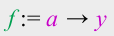
\includegraphics[scale=0.8]{tutorials/figures/palettefunc.png}
\caption{You can find a shortcut for defining functions in the palettes toolbar under Expression. This button makes use of the arrow notation.}
\end{marginfigure}

\section{Using Function Notation}
\label{sec:function_notation}

Once we have defined a function, we can use function notation much like we would in class. For example, instead of defining an expression involving $x$ to a name such as \texttt{expr} and then using the \texttt{subs()} command to substitute $x=0$ into \texttt{expr}, we can now use the function $f(x)$ as assigned in Section \ref{sec:define_function} and type $f(0)$.

\begin{maplegroup}
\begin{mapleinput}
\mapleinline{active}{1d}{f(0);
}{}
\end{mapleinput}
\mapleresult
\begin{maplelatex}
\mapleinline{inert}{2d}{-1}{\[\displaystyle -1\]}
\end{maplelatex}
\end{maplegroup}

It is easy to substitute an expression into a function using function notation.

\begin{maplegroup}
\begin{mapleinput}
\mapleinline{active}{1d}{g(x) := 2*x\symbol{94}2 - 3*x;
}{}
\end{mapleinput}
\mapleresult
\begin{maplelatex}
\mapleinline{inert}{2d}{g := proc (x) options operator, arrow; 2*x^2-3*x end proc}{\[\displaystyle g\, := \,x\mapsto 2\,{x}^{2}-3\,x\]}
\end{maplelatex}
\end{maplegroup}

\begin{maplegroup}
\begin{mapleinput}
\mapleinline{active}{1d}{g(x+1);
}{}
\end{mapleinput}
\mapleresult
\begin{maplelatex}
\mapleinline{inert}{2d}{2*(x+1)^2-3*x-3}{\[\displaystyle 2\, \left( x+1 \right) ^{2}-3\,x-3\]}
\end{maplelatex}
\end{maplegroup}

\section{Operations on Functions}
\label{sec:operations_on_functions}

Once one or more functions are assigned, we can make expressions using function notation, or perform other operations on those functions.

\begin{maplegroup}
\begin{mapleinput}
\mapleinline{active}{1d}{f(x) := 2*x\symbol{94}3;
}{}
\end{mapleinput}
\mapleresult
\begin{maplelatex}
\mapleinline{inert}{2d}{f := proc (x) options operator, arrow; 2*x^3 end proc}{\[\displaystyle f\, := \,x\mapsto 2\,{x}^{3}\]}
\end{maplelatex}
\end{maplegroup}
\begin{maplegroup}
\begin{mapleinput}
\mapleinline{active}{1d}{g(t) := t+1;
}{}
\end{mapleinput}
\mapleresult
\begin{maplelatex}
\mapleinline{inert}{2d}{g := proc (t) options operator, arrow; t+1 end proc}{\[\displaystyle g\, := \,t\mapsto t+1\]}
\end{maplelatex}
\end{maplegroup}
\begin{maplegroup}
\begin{mapleinput}
\mapleinline{active}{1d}{f(g(t)); expand(%);
}{}
\end{mapleinput}
\mapleresult
\begin{maplelatex}
\mapleinline{inert}{2d}{2*(t+1)^3}{\[\displaystyle 2\, \left( t+1 \right) ^{3}\]}
\end{maplelatex}
\mapleresult
\begin{maplelatex}
\mapleinline{inert}{2d}{2*t^3+6*t^2+6*t+2}{\[\displaystyle 2\,{t}^{3}+6\,{t}^{2}+6\,t+2\]}
\end{maplelatex}
\end{maplegroup}
\begin{maplegroup}
\begin{mapleinput}
\mapleinline{active}{1d}{plot(f(x), x=-5..5);
}{}
\end{mapleinput}
\mapleresult
\mapleplot{tutorials/figures/funtionnotationplot2d1-eps-converted-to.pdf}
\end{maplegroup}

\index{expand}
\index{plot}
\index{plot!axes intervals}

\subsection{Average Rate of Change of a Function over an Interval}

In this example, we will find the average rate of change of the function $f(x) = -2x^3 + 25x^2 + 15$ over the interval $[2,7]$. We begin by defining the function:

\begin{maplegroup}
\begin{mapleinput}
\mapleinline{active}{1d}{f(x) := -2*x\symbol{94}3 + 25*x\symbol{94}2 + 15;
}{}
\end{mapleinput}
\mapleresult
\begin{maplelatex}
\mapleinline{inert}{2d}{f := proc (x) options operator, arrow; -2*x^3+25*x^2+15 end proc}{\[\displaystyle f\, := \,x\mapsto -2\,{x}^{3}+25\,{x}^{2}+15\]}
\end{maplelatex}
\end{maplegroup}

Once the function is defined, we can calculate the average rate of change over an interval $[a,b]$ by using the formula \[ \frac{f(b)-f(a)}{b-a}. \] 
In this case, we let $a=2$ and $b=7$:

\marginnote{This fraction will look much nicer on your screen if you use 2D Math font.}
\begin{maplegroup}
\begin{mapleinput}
\mapleinline{active}{1d}{(f(7) - f(2))/(7 - 2);
}{}
\end{mapleinput}
\mapleresult
\begin{maplelatex}
\mapleinline{inert}{2d}{91}{\[\displaystyle 91\]}
\end{maplelatex}
\end{maplegroup}
\begin{maplegroup}
\begin{mapleinput}
\mapleinline{active}{1d}{}{}
\end{mapleinput}
\end{maplegroup}

\noindent
The average rate of change over the interval $[2,7]$ is $91$. The units of this rate would be given in (units of $y$)/(units of $x$).

\subsection{Plotting Transformations of Functions}
\label{subsec:plotting_transformations}

Suppose that we start with a sinusoidal function $g(x)$ with amplitude $2$ and period $2$.

\begin{maplegroup}
\begin{mapleinput}
\mapleinline{active}{1d}{g(x) := 2*sin(Pi*x);
}{}
\end{mapleinput}
\end{maplegroup}

\begin{maplegroup}
\begin{mapleinput}
\mapleinline{active}{1d}{plot(g(x), x=0..4, y=-4..4);
}{}
\end{mapleinput}
\mapleresult
\mapleplot{tutorials/figures/transformationsplot2d1-eps-converted-to.pdf}
\end{maplegroup}

\index{plot}
\index{Pi}
\index{plot!axes intervals}
\index{plot!multiple functions}

We can then plot the original function $g(x)$ and and the transformation $\frac{1}{2}g(x)$ on the same axes to see that the amplitude has been halved.

\begin{maplegroup}
\begin{mapleinput}
\mapleinline{active}{1d}{plot([g(x), 0.5*g(x)], x=0..4, y=-4..4);
}{}
\end{mapleinput}
\mapleresult
\mapleplot{tutorials/figures/transformationsplot2d2-eps-converted-to.pdf}
\end{maplegroup}

We can also see how an absolute value transformation of $g(x)$ compares to the original function. The result here is known as a fully rectified sine wave.

\begin{maplegroup}
\begin{mapleinput}
\mapleinline{active}{1d}{plot([ g(x), abs(g(x)) ], x=0..4, y=-4..4);
}{}
\end{mapleinput}
\mapleresult
\mapleplot{tutorials/figures/transformationsplot2d3-eps-converted-to.pdf}
\end{maplegroup}

\index{mathematical functions!absolute value}
\index{plot!axes intervals}
\index{plot!multiple functions}

\section{Assigning Piecewise Functions}
\label{sec:piecewise}

A piecewise-defined function is a function defined by multiple sub-functions. Each sub-function applies to a certain interval of the domain, called a sub-domain. We can define piecewise functions in Maple by using the \texttt{piecewise()} command. The sub-domain of each sub-function is specified before its expression.

\index{mathematical functions!piecewise}

\begin{maplegroup}
\begin{mapleinput}
\mapleinline{active}{1d}{P(x) := piecewise(x<=-1, x\symbol{94}2, -1<x<=1, -x, 1<x, x-4);
}{}
\index{mathematical functions!piecewise}
\end{mapleinput}
\mapleresult
\begin{maplelatex}
\mapleinline{inert}{2d}{P := proc (x) options operator, arrow; piecewise(x <= -1, x^2, -1 < x <= 1, -x, 1 < x, x-4) end proc}{\[\displaystyle P\, := \,x\mapsto \begin{cases}{x}^{2}&x\leq -1 \\ -x&-1< x\leq 1 \\ x-4&1<x\end{cases}\]}
\end{maplelatex}
\end{maplegroup}

\begin{maplegroup}
\begin{mapleinput}
\mapleinline{active}{1d}{P(x);
}{}
\end{mapleinput}
\mapleresult
\begin{maplelatex}
\mapleinline{inert}{2d}{piecewise(x <= -1, x^2, -1 < x <= 1, -x, 1 < x, x-4)}{\[\displaystyle \begin{cases}{x}^{2}& x\leq -1 \\ -x& -1 < x\leq 1 \\ x-4&1<x\end{cases}\]}
\end{maplelatex}
\end{maplegroup}

\section{Functions of More than One Variable}
\label{sec:functions_multiple_variables}

We can also define functions of multiple variables and use the notation the same way as one variable functions.

\index{mathematical functions!sine}
\index{mathematical functions!cosine}
\index{mathematical functions!multivariable functions}

\begin{maplegroup}
\begin{mapleinput}
\mapleinline{active}{1d}{g(x,y) := sin(x) - cos(y);
}{}
\end{mapleinput}
\mapleresult
\begin{maplelatex}
\mapleinline{inert}{2d}{g := proc (x, y) options operator, arrow; sin(x)-cos(y) end proc}{\[\displaystyle g\, := \,( {x,y} )\mapsto \sin \left( x \right) -\cos \left( y \right) \]}
\end{maplelatex}
\end{maplegroup}

\noindent
Evaluating at a point:

\begin{maplegroup}
\begin{mapleinput}
\mapleinline{active}{1d}{g(0, Pi);
}{}
\end{mapleinput}
\mapleresult
\begin{maplelatex}
\mapleinline{inert}{2d}{1}{\[\displaystyle 1\]}
\end{maplelatex}
\end{maplegroup}

\index{Pi}

An example of a function of more than one variable is the volume of a circular cylinder.

\begin{maplegroup}
\begin{mapleinput}
\mapleinline{active}{1d}{cylindervol(r,h) := Pi*r\symbol{94}2*h;
}{}
\end{mapleinput}
\mapleresult
\begin{maplelatex}
\mapleinline{inert}{2d}{cylindervol := proc (r, h) options operator, arrow; Pi*r^2*h end proc}{\[\displaystyle {\it cylindervol}\, := \,( {r,h} )\mapsto \pi\,{r}^{2}h\]}
\end{maplelatex}
\end{maplegroup}

\begin{maplegroup}
\begin{mapleinput}
\mapleinline{active}{1d}{cylindervol(3,5);
}{}
\end{mapleinput}
\mapleresult
\begin{maplelatex}
\mapleinline{inert}{2d}{45*Pi}{\[\displaystyle 45\,\pi\]}
\end{maplelatex}
\end{maplegroup}

\section{Assigning Plots and the \texttt{display()} Command}
\label{sec:display_command}

You can use the assignment operator to assign just about any type of output to a variable name, including plots. This can be useful when different types of plots need to be displayed on the same graph. You can assign the output of several \texttt{plot()} commands to variables and then 'display' them all on the same set of axes. 

To make use of the \texttt{display()} command, you need to include the \texttt{plots} package. Packages are loaded using the \texttt{with()} command, where the name of the package appears within the parentheses. The command
\index{packages!plots}
\index{packages!with}
\begin{maplegroup}
\begin{mapleinput}
\mapleinline{active}{1d}{with(plots);
}{}
\end{mapleinput}
\mapleresult
\begin{maplelatex}
\mapleinline{inert}{2d}{[plots:-animate, plots:-animate3d, plots:-animatecurve, plots:-arrow, plots:-changecoords, plots:-complexplot, plots:-complexplot3d, plots:-conformal, plots:-conformal3d, plots:-contourplot, plots:-contourplot3d, plots:-coordplot, plots:-coordplot3d, plots:-densityplot, plots:-display, plots:-dualaxisplot, plots:-fieldplot, plots:-fieldplot3d, plots:-gradplot, plots:-gradplot3d, plots:-implicitplot, plots:-implicitplot3d, plots:-inequal, plots:-interactive, plots:-interactiveparams, plots:-intersectplot, plots:-listcontplot, plots:-listcontplot3d, plots:-listdensityplot, plots:-listplot, plots:-listplot3d, plots:-loglogplot, plots:-logplot, plots:-matrixplot, plots:-multiple, plots:-odeplot, plots:-pareto, plots:-plotcompare, plots:-pointplot, plots:-pointplot3d, plots:-polarplot, plots:-polygonplot, plots:-polygonplot3d, plots:-polyhedra_supported, plots:-polyhedraplot, plots:-rootlocus, plots:-semilogplot, plots:-setcolors, plots:-setoptions, plots:-setoptions3d, plots:-shadebetween, plots:-spacecurve, plots:-sparsematrixplot, plots:-surfdata, plots:-textplot, plots:-textplot3d, plots:-tubeplot]}{\[\displaystyle [{\it animate},{\it animate3d},{\it animatecurve}
\hdots
\mbox{}]\]}
\end{maplelatex}
\end{maplegroup}
\noindent
will display all of the commands that are included in the package. If a full colon is added, then the package is loaded but the output is hidden.

\begin{maplegroup}
\begin{mapleinput}
\mapleinline{active}{1d}{with(plots):
}{}
\end{mapleinput}
\end{maplegroup}

With the \texttt{plots} package loaded, plotting options can be defined for each plot individually and assigned to a name. Multiple plots can then be displayed together.

\marginnote{A package does not need to be loaded more than once in your document. However, you will need to reload the package if you have previously closed the document.}
\begin{maplegroup}
\begin{mapleinput}
\mapleinline{active}{1d}{p1(x) := (x+2)\symbol{94}2 + 2*(x+2) - 5;
p2(x) := 3*(x-4)\symbol{94}3 - 2*(x-4)\symbol{94}2 - (x-4) + 1;
p3(x) := x - 3;
}{}
\end{mapleinput}
\mapleresult
\begin{maplelatex}
\mapleinline{inert}{2d}{p1 := proc (x) options operator, arrow; (x+2)^2+2*x-1 end proc}{\[\displaystyle {\it p1}\, := \,x\mapsto  \left( x+2 \right) ^{2}+2\,x-1\]}
\end{maplelatex}
\mapleresult
\begin{maplelatex}
\mapleinline{inert}{2d}{p2 := proc (x) options operator, arrow; 3*(x-4)^3-2*(x-4)^2-x+5 end proc}{\[\displaystyle {\it p2}\, := \,x\mapsto 3\, \left( x-4 \right) ^{3}-2\, \left( x-4 \right) ^{2}-x+5\]}
\end{maplelatex}
\mapleresult
\begin{maplelatex}
\mapleinline{inert}{2d}{p3 := proc (x) options operator, arrow; x-3 end proc}{\[\displaystyle {\it p3}\, := \,x\mapsto x-3\]}
\end{maplelatex}
\end{maplegroup}

\index{plot}
\index{plot!axes intervals}
\index{plot!line style}
\index{display}

\marginnote[0.5cm]{Full colons are used at the end of each line here to hide the output of the individual plot.}
\begin{maplegroup}
\begin{mapleinput}
\mapleinline{active}{1d}{A := plot(p1(x), x=-6..0, y=-6..3, linestyle=dot):
}{}
\end{mapleinput}
\end{maplegroup}
\begin{maplegroup}
\begin{mapleinput}
\mapleinline{active}{1d}{B := plot(p2(x), x=-0..10, y=-10..10, style=point):
}{}
\end{mapleinput}
\end{maplegroup}
\begin{maplegroup}
\begin{mapleinput}
\mapleinline{active}{1d}{C := plot(p3(x), x=-10..10, y=-10..10):
}{}
\end{mapleinput}
\end{maplegroup}
\begin{maplegroup}
\begin{mapleinput}
\mapleinline{active}{1d}{display([A,B,C]);
}{}
\end{mapleinput}
\mapleresult
\mapleplot{tutorials/figures/Plotting_Functionsplot2d4-eps-converted-to.pdf}
\end{maplegroup}
\begin{maplegroup}
\begin{mapleinput}
\mapleinline{active}{1d}{}{}
\end{mapleinput}
\end{maplegroup}
\begin{Maple Normal}{
\begin{Maple Normal}{
\mapleinline{inert}{2d}{}{\[\displaystyle \]}
}\end{Maple Normal}
}\end{Maple Normal}
\begin{Maple Normal}{
\begin{Maple Normal}{
\mapleinline{inert}{2d}{}{\[\displaystyle \]}
}\end{Maple Normal}
}\end{Maple Normal}